\section{随机变量及其分布}
分布函数变量区域左闭右开,概率密度则不要求。

\subsection{分布概念}

\paragraph{\boxed{\text{分布函数存在性}}}

分布函数的充要条件是:

\begin{enumerate}
    \item $F(x)$单调不减。
    \item $\lim\limits_{x\to-\infty}F(x)=0$。
    \item $\lim\limits_{x\to+\infty}F(x)=1$。
    \item $F(x)$右连续。
\end{enumerate}

这也是下面的计算需要考虑的性质。

\textbf{例题:}设随机变量$X$的分布函数$F(x)$,判断$F(ax)$、$F(x^2+1)$、$F(x^3-1)$、$F(\vert X\vert)$是否可以做出分布函数。

解:逐个分析$F(g(x))$中的$g(x)$走向。

$\lim\limits_{x\to+\infty}F(ax)=a\lim\limits_{x\to+\infty}F(x)=a$,不满足。

由于$x^2+1$在$x\to-\infty$的趋向为$+\infty$而不是$-\infty$,$\lim\limits_{x\to-\infty}F(x^2+1)=\lim\limits_{x\to+\infty}F(x^2+1)=\lim\limits_{x\to-\infty}F(x)=1\neq0$,不满足。

$F(x^3-1)$满足分布函数的四个条件,$g(x)=x^3-1$在两边趋向与原函数一致。

$F(\vert x\vert)$的$g(x)=\vert x\vert$在$x\to-\infty$的趋向为$+\infty$而不是$-\infty$,不满足$\lim\limits_{x\to-\infty}F(x)=0$,不满足。

\paragraph{\boxed{\text{分布函数计算}}}

这里所说的分布函数都是不定式,需要利用分布函数性质来换算。

\textbf{例题:}随机变量$X$的概率密度函数$f(x)$满足$f(1+x)=f(1-x)$,且$\int_1^2f(x)\,\textrm{d}x=0.3$,则求分布函数$F(0)$的值。

解:已知$f(1+x)=f(1-x)$,所以$f(x)$关于$x=1$对称。所以$\int_1^{+\infty}f(x)\,\textrm{d}x=\int_1^{-\infty}f(x)\,\textrm{d}x=\dfrac{1}{2}$。

所以$\int_1^2f(x)\,\textrm{d}x=\int_0^1f(x)\,\textrm{d}x=0.3$。

$F(0)=\int_{-\infty}^0f(x)\,\textrm{d}x=1-\int_0^{+\infty}f(x)\,\textrm{d}x=1-\int_1^{+\infty}f(x)\,\textrm{d}x-\int_0^1f(x)\,\textrm{d}x=0.2$。

\paragraph{\boxed{\text{概率密度存在性}}}

分布函数的充要条件是:

\begin{enumerate}
    \item $f(x)\geqslant0$。
    \item $\int_{-\infty}^{+\infty}f(x)\,\textrm{d}x=1$。
\end{enumerate}

\textbf{例题:}随机变量$X$的概率密度函数$f(x)$,判断$f(2x)$、$f(2-x)$是否可以作出概率密度函数。

解:$\int_{-\infty}^{+\infty}f(2x)\,\textrm{d}x=\dfrac{1}{2}\int_{-\infty}^{+\infty}f(2x)\,\textrm{d}(2x)=\dfrac{1}{2}\neq1$,不满足。

$\int_{-\infty}^{+\infty}f(2-x)\,\textrm{d}x=-\int_{-\infty}^{+\infty}f(2-x)\,\textrm{d}(2-x)$,令$2-x=t$,则$x\to-\infty$时$t\to+\infty$,$x\to+\infty$时$t\to-\infty$,$=-\int_{+\infty}^{-\infty}f(t)\,\textrm{d}t=\int_{-\infty}^{+\infty}f(t)\,\textrm{d}t=1$。

\paragraph{\boxed{\text{概率密度计算}}}

\textbf{例题:}随机变量$X$的分布函数和概率密度函数为$F(x)$,$f(x)$,求$-X$的分布函数和概率密度。

解:已知$F(x)=P\{X\leqslant x\}$,则$F'(-x)=\{-X\leqslant x\}$,即$F'(-x)=P\{X\geqslant-x\}=1-P\{X\leqslant-x\}=1-F(-x)$。

对$F'(-x)$进行求导:$[1-F(-x)]'=f(-x)$。

\textbf{例题:}随机变量$X$的概率密度为$f(x)$,求随机变量$2X+3$的概率密度函数。

解:设$Y=2X+3$,所以$Y$的分布函数$F_Y(y)$为$F_Y(x)=P\{Y\leqslant x\}=P\{2X+3\leqslant x\}=P\left\{X\leqslant\dfrac{x-3}{2}\right\}=\int_{-\infty}^{\frac{t-3}{2}}f(x)\,\textrm{d}x$。

所以其概率密度为$f_Y(x)=(\int_{-\infty}^{\frac{x-3}{2}}f(x)\,\textrm{d}x)'=\dfrac{1}{2}f\left(\dfrac{x-3}{2}\right)$。

\subsection{一维随机变量}

\paragraph{\boxed{\text{一维随机变量分布}}}

\subsubsection{二项分布}

$P\{X=k\}=C_n^kp^k(1-p)^{n-k}$($k=0,1,\cdots,n$,$0<p<1$),$X\sim B(n,p)$。

\textbf{例题:}已知随机变量$X$的概率密度为$f(x)=\left\{\begin{array}{ll}
    2x, & 0<x<1 \\
    0, \text{其他}
\end{array}\right.$,$Y$表示对$X$进行3次独立重复试验中出现事件$\left\{X\leqslant\dfrac{1}{2}\right\}$,求$P\{Y=2\}$。\medskip

解:已知对$X$进行独立重复试验,表示这个进行的是伯努利试验,从而$Y\sim B(n,p)$。又是3次,所以$Y\sim B(3,p)$。

只用求出这个$p$即$\left\{X\leqslant\dfrac{1}{2}\right\}$的概率就可以了。又已知$f(x)$。

$\therefore p=\left\{X\leqslant\dfrac{1}{2}\right\}=\int_0^\frac{1}{2}2x\,\textrm{d}x=\dfrac{1}{4}$。$\therefore P\{Y=2\}=B\left(3,\dfrac{1}{4}\right)=\dfrac{9}{64}$。

\subsubsection{泊松分布}

$P\{X=k\}=\dfrac{\lambda^k}{k!}e^{-\lambda}$($k=0,1,\cdots,n$,$\lambda>0$),$X\sim P(\lambda)$。

\textbf{例题:}设一本书的各页印刷错误的个数$X$服从泊松分布。已知只有一个和只有两个印刷错误的页数相同,则随机抽查的4页中无印刷错误的概率$p$为?

解:$\because P\{X=1\}=P\{X=2\}$,$\therefore\dfrac{\lambda^1}{1!}e^{-\lambda}=\dfrac{\lambda^2}{2!}e^{-\lambda}$,$\lambda=2$。

由于随机抽四页类似于伯努利试验是相互独立的,所以随机抽4页都无错误的概率为$[P\{X=0\}]^4=e^{-8}$。

\subsubsection{几何分布}

$P\{X=k\}=(1-p)^{k-1}p$($k=0,1,\cdots,n$,$0<p<1$),$X\sim G(p)$。

\textbf{例题:}袋中有8个球,其中3个白球5个黑球,现在任意从中取出4个球,若四个球中有2个黑球和2个白球则试验停止,否则将其放回袋中重新抽取直到满足条件,用$X$表示试验次数,则求$P\{X=k\}$。

解:由题目的停止,则说明这个题目的概率是服从几何分布的,最重要的就是求出单次满足事件概率$p$。

根据组合和乘法原理,$p=\dfrac{C_3^2C_5^2}{C_8^4}=\dfrac{3}{7}$。

则$P\{X=k\}=\left(\dfrac{4}{7}\right)^{k-1}\cdot\dfrac{3}{7}$。

\textbf{例题:}已知随机变量$X$的概率密度为$f(x)=\left\{\begin{array}{ll}
    2^{-x}\ln2, & x>0 \\
    0, \text{其他}
\end{array}\right.$,对$X$进行独立重复观测,直到第2个大于3的观测值出现时停止,记$Y$为观测次数,求$Y$的概率分布。

解:由题目直到就停止,知道$Y\sim G(p)$。

又$p=P\{X\geqslant3\}=\int_3^{+\infty}2^{-x}\ln2\,\textrm{d}x=\dfrac{1}{8}$

这是对几何分布的变形,首先进行$k$次试验,第$k$次成功,所以要乘$p$,而因为是第2个成功,所以前面的$k-1$次中有$k-2$次失败和一次成功,所以一共$p^2(1-k)^{k-2}$。因为前面的成功的一次在$k-1$中任意一个地方就可以了,所以一共有$k-1$中可能性,要考虑到排列,所以还要乘$(k-1)$。

$\therefore P\{Y=k\}=(k-1)\left(\dfrac{1}{8}\right)^2\cdot\left(\dfrac{7}{8}\right)^{k-2}$。

\subsubsection{均匀分布}

$f(x)=\left\{\begin{array}{ll}
    \dfrac{1}{b-a}, & a<x<b \\
    0, & \text{其他}
\end{array}\right.$,$F(x)=\left\{\begin{array}{ll}
    0, & x<a \\
    \dfrac{x-a}{b-a}, & a\leqslant x<b \\
    1, & x\geqslant b
\end{array}\right.$,$X\sim U(a,b)$。

\textbf{例题:}已知随机变量$X\sim U(a,b)$($a>0$)且$P\{0<X<3\}=\dfrac{1}{4}$,$P\{X>4\}=\dfrac{1}{2}$,求$X$的概率密度以及$P\{1<X<5\}$。

解:$\because P\{X>4\}=\dfrac{1}{2}$,4在其区间中点上,$\dfrac{a+b}{2}=4$。

$\because P\{0<X<3\}=\dfrac{1}{4}$,$3$若在$a$左边则概率为0,所以必然在右边。

$\therefore P\{a<X<3\}=\dfrac{1}{4}$,$P\{<3X<4\}=1-\dfrac{1}{4}-\dfrac{1}{2}=\dfrac{1}{4}$,$\dfrac{4-3}{b-a}=\dfrac{1}{4}$。

解得$a=2$,$b=6$,$X\sim U(2,6)=f(x)=\left\{\begin{array}{ll}
    \dfrac{1}{4}, & 2<x<6 \\
    0, & \text{其他}
\end{array}\right.$。

$P\{1<X<5\}=\dfrac{5-2}{6-2}=\dfrac{3}{4}$。

\textbf{例题:}已知随机变量$X$在区间$[0,1]$上服从均匀分布,在$X=x$($0<x<1$)的条件下随机变量$Y$在区间$[0,x]$上服从均匀分布。

(1)$(X,Y)$的概率密度。

解:$X$在区间$[0,1]$上服从均匀分布,则$X\sim f_X(x)=\left\{\begin{array}{ll}
    1, & 0\leqslant x\leqslant1 \\
    0, & \text{其他}
\end{array}\right.$。

$Y$在$X=x$下均匀分布,则$f_{Y|X}(y|x)=\left\{\begin{array}{ll}
    \dfrac{1}{x}, & 0<y<x<1 \\
    0, & \text{其他}
\end{array}\right.$。

$(X,Y)$联合概率=条件概率×边缘概率。

即$f(x,y)=f_{Y|X}(y|x)f_X(x)=\left\{\begin{array}{ll}
    \dfrac{1}{x}, & 0<y<x<1 \\
    0, & \text{其他}
\end{array}\right.$。

(2)$Y$的概率密度。

解:首先求$Y$的边缘概率密度,就需要积$X$。然后求$y$的区间,$XY$的联合区间是横坐标$[0,1]$到纵坐标$[0,1]$的下三角形,则$y\in[0,1]$。

然后求$Y$就在联合概率密度所规定的区间中画一条$y=y_0$的线,从左先交到的是$y=x$,所以下限就是$y$,后交的是$x=1$,所以上限为1。最后将$y$的联合分布函数放在中间,得到$f_Y(y)=\left\{\begin{array}{ll}
    \displaystyle{\int_y^1\dfrac{1}{x}\textrm{d}x}=-\ln y, & 0<y<x<1 \\
    0, & \text{其他}
\end{array}\right.$。

(3)概率$P\{X+Y>1\}$。

解:求$P\{X+Y>1\}$就是求一个区间的概率值,即$P\{(X,Y)\in G\}=\iint\limits_Gf(x,y)\,\textrm{d}x\textrm{d}y$。

\begin{multicols}{2}
    
    \begin{tikzpicture}[scale=2]
        \draw[-latex](-0.25,0) -- (1.25,0) node[below]{$x$};
        \draw[-latex](0,-0.25) -- (0,1.25) node[above]{$y$};
        \filldraw[black] (0,0) node[below]{$O$};
        \draw[black](1,0) -- (0,1) node[left]{$1$};
        \draw[black](1,1) -- (1,0) node[below]{$1$};
        \draw[black](0,0) -- (1,1);
        \draw[black, densely dashed](0.5,0.5) -- (0.5,0) node[below]{$\dfrac{1}{2}$};
        \filldraw [fill=gray!20] (0.5,0.5) -- (1,1) -- (1,0) -- (0.5,0.5);
        \draw[black](0.8,0.5) node{$D$};
        \draw[black, densely dashed](0.6,0) -- (0.6,1) node[above]{$y=y_0$};
    \end{tikzpicture}

    所以$P\{X+Y>1\}=\iint\limits_D\dfrac{1}{x}\textrm{d}\sigma$,$D=x+y>1\cap0<y<x<1$。$\iint\limits_D\dfrac{1}{x}\,\textrm{d}\sigma=\int_\frac{1}{2}^1\textrm{d}x\int_{1-x}^x\dfrac{1}{x}\textrm{d}y=1-\ln2$。

\end{multicols}

\subsubsection{指数分布}

$f(x)=\left\{\begin{array}{ll}
    \lambda e^{-\lambda x}, & x>0 \\
    0, & \text{其他}
\end{array}\right.$,$F(x)=\left\{\begin{array}{ll}
    1-e^{-\lambda x}, & x\geqslant0 \\
    0, & x<0 \\
\end{array}\right.$,$X\sim E(\lambda)$。

\textbf{例题:}已知随机变量$X\sim E(1)$,$a$为常数且大于0,求$P\{X\leqslant a+1|X>a\}$。

解:$P\{X\leqslant a+1|X>a\}=\dfrac{P\{a<X\leqslant a+1\}}{P\{X>a\}}=\dfrac{\int_a^{a+1}e^{-x}\,\textrm{d}x}{\int_a^{+\infty}e^{-x}\,\textrm{d}x}=1-\dfrac{1}{e}$。

也可以根据指数分布的无记忆性:$P\{X\leqslant a+1|X>a\}=1-P\{X>a+1|X>a\}=1-P\{X>1\}=P\{X\leqslant1\}=F(1)=1-\dfrac{1}{e}$。

\textbf{例题:}随机变量$X$服从参数为1的指数分布,求$P\{3>X>2|X>1\}$。

已知$F(X<x)=1-e^{-\lambda x}$,则$F(X>x)=e^{-\lambda x}$。且$2<X<3\cap 1<X=2<X<3$。

则$P\{3>X>2|X>1\}=\dfrac{P\{3>X>2\}}{P\{X>1\}}=\dfrac{P\{X>2\}-P\{X>3\}}{P\{X>1\}}=\dfrac{e^{-2}-e^{-3}}{e^{-1}}=e^{-1}-e^{-2}$。

\subsubsection{正态分布}

$f(x)=\dfrac{1}{\sqrt{2\pi}\sigma}e^{-\frac{(x-\mu)^2}{2\sigma^2}}$($-\infty<x<+\infty$,$-\infty<\mu<+\infty$,$\sigma>0$),$X\sim N(\mu,\sigma^2)$。

\textbf{例题:}已知随机变量$X\sim N(0,1)$,对给定的$\alpha$($0<\alpha>1$),数$\mu_\alpha$满足$P\{X>\mu_\alpha\}=\alpha$,若$P\{\vert X\vert<x\}=\alpha$,求$x$。

解:$P\{X>\mu_\alpha\}=\alpha$即表示$\mu_\alpha$为标准正态分布的上$\alpha$分位点。

又$P\{\vert X\vert<x\}=\alpha$,即$-x<X<x$的面积为$\alpha$,所以两边的面积各为$\dfrac{1-\alpha}{2}$,$P\{X<x\}=P\{X>x\}=\dfrac{1-\alpha}{2}$。

$\because$面积为$\alpha$的下标为$\alpha$,$\therefore$面积为$\dfrac{1-\alpha}{2}$的下标为$\dfrac{1-\alpha}{2}$,$x=\mu_\frac{1-\alpha}{2}$。

\paragraph{\boxed{\text{一维随机变量函数分布}}}

\textbf{例题:}随机变量$X$服从$U(0,2)$,求随机变量$Y=X^2$在$(0,4)$内的概率分布密度$f_Y(y)$。

解:求概率分布密度函数,可以求出其积分概率分布函数,$F_Y(y)=P\{Y\leqslant y\}=P\{X^2\leqslant y\}=P\{-\sqrt{y}\leqslant X\leqslant\sqrt{y}\}$,又$X\sim U(0,2)$,所以$f(x)=\dfrac{1}{2}$。

则概率分布函数就是概率密度的积分,此时已经将$Y$变为了关于$X$的积分,$=\int_{-\sqrt{y}}^{\sqrt{y}}f(x)\,\textrm{d}x=$$\displaystyle{2\int_0^{\sqrt{y}}\dfrac{1}{2}\,\textrm{d}x}=\dfrac{\sqrt{y}}{2}$。即$F_Y(y)=\dfrac{\sqrt{y}}{2}$。

则$f_Y(y)=F'_Y(y)=\dfrac{1}{4\sqrt{y}}$。

\subsection{二维随机变量}

使用定义法则直接用二重积分的分布函数来求,使用卷积公式则使用概率密度。

\paragraph{\boxed{\text{二维离散型随机变量}}}

\paragraph{\boxed{\text{二维连续型随机变量}}}

有两种主要方法,一个是分布函数法,一个是卷积公式法。如果给出联合概率密度使用分布函数法,如果给出边缘概率密度使用卷积公式法。

\subsubsection{联合概率}

\paragraph{\boxed{\text{联合概率密度}}} \leavevmode \medskip

利用联合概率函数来计算,有两种方式,一种是以概率形式,一种是以积分形式。

\textbf{例题:}已知二维随机变量$(X_1,X_2)$的概率密度函数$f_1(x_1,x_2)$,求$Y_1=2X_1$,$Y_2=\dfrac{1}{3}X_2$的联合概率密度$f_2(y_1,y_2)$。

解:概率形式:设$F_2(y_1,y_2)=P\{Y_1\leqslant y_1,Y_2\leqslant y_2\}=P\{2X_1\leqslant y_1,\dfrac{1}{3}X_2\leqslant y_2\}=P\{X_1\leqslant\dfrac{y_1}{2},X_2\leqslant3y_2\}=F_1(\dfrac{y_1}{2},3y_2)$。所以$f_2(y_1,y_2)=\dfrac{3}{2}f_1(\dfrac{y_1}{2},3y_2)$。

积分形式:已知$\int_{-\infty}^{+\infty}\textrm{d}x_1\int_{-\infty}^{+\infty}f(x_1,x_2)\,\textrm{d}x_2=1$,将$x_1=\dfrac{y_1}{2}$,$x_2=3y_2$代入$\int_{-\infty}^{+\infty}\textrm{d}(\dfrac{y_1}{2})\int_{-\infty}^{+\infty}f(\dfrac{y_1}{2},3y_2)\,\textrm{d}(3y_2)=1$,$\dfrac{3}{2}\int_{-\infty}^{+\infty}\textrm{d}y_1\int_{-\infty}^{+\infty}f(\dfrac{y_1}{2},3y_2)\,\textrm{d}y_2=1$,所以$f_2(y_1,y_2)=\dfrac{3}{2}f_1(\dfrac{y_1}{2},3y_2)$。

\paragraph{\boxed{\text{联合概率函数}}} \leavevmode \medskip

已知联合概率密度,可以求概率函数,通过二重积分的方式,图像面积即是概率。

\textbf{例题:}已知概率密度为$f(x,y)=\left\{\begin{array}{ll}
    6, & 0<x^2<y<x<1 \\
    0, & \text{其他}
\end{array}\right.$,\\求$P\left\{X>\dfrac{1}{2}\right\}$,$P\left\{Y<\dfrac{1}{2}\right\}$。

解:

\begin{minipage}{0.45\linewidth}
    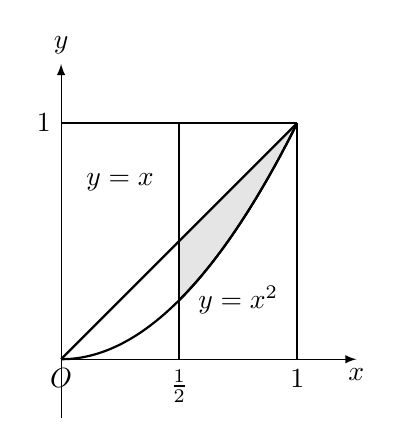
\begin{tikzpicture}[scale=3]
        \begin{scope}
            \clip(0.5,0)rectangle(1,1);
            \draw[black, thick, smooth, domain=0:1,fill=gray!20] plot (\x, {\x*\x});
        \end{scope}
        \draw[black, thick, smooth, domain=0:1] plot (\x, {\x*\x});
        \draw[black, thick, smooth, domain=0:1] plot (\x, {\x});
        \draw[black, thick](1/2,1) -- (1/2,0) node[below]{$\frac{1}{2}$};
        \draw[-latex](0,0) -- (1.25,0) node[below]{$x$};
        \draw[-latex](0,-0.25) -- (0,1.25) node[above]{$y$};
        \filldraw[black] (0,0) node[below]{$O$};
        \draw[black, thick](1,1) -- (0,1) node[left]{$1$};
        \draw[black, thick](1,1) -- (1,0) node[below]{$1$};
        \filldraw[black] (0.25,0.75) node{$y=x$};
        \filldraw[black] (0.75,0.25) node{$y=x^2$};
    \end{tikzpicture}
\end{minipage}
\hfill
\begin{minipage}{0.45\linewidth}
    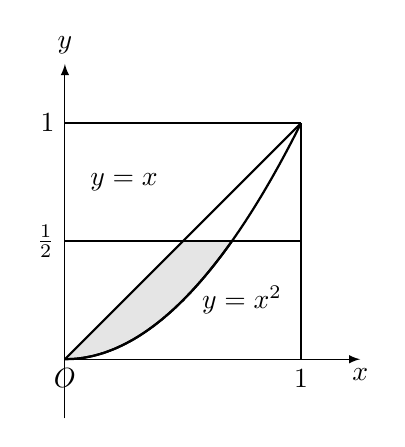
\begin{tikzpicture}[scale=3]
        \begin{scope}
            \clip(0,0)rectangle(1,0.5);
            \draw[black, thick, smooth, domain=0:1,fill=gray!20] plot (\x, {\x*\x});
        \end{scope}
        \draw[black, thick, smooth, domain=0:1] plot (\x, {\x*\x});
        \draw[black, thick, smooth, domain=0:1] plot (\x, {\x});
        \draw[black, thick](1,1/2) -- (0,1/2) node[left]{$\frac{1}{2}$};
        \draw[-latex](0,0) -- (1.25,0) node[below]{$x$};
        \draw[-latex](0,-0.25) -- (0,1.25) node[above]{$y$};
        \filldraw[black] (0,0) node[below]{$O$};
        \draw[black, thick](1,1) -- (0,1) node[left]{$1$};
        \draw[black, thick](1,1) -- (1,0) node[below]{$1$};
        \filldraw[black] (0.25,0.75) node{$y=x$};
        \filldraw[black] (0.75,0.25) node{$y=x^2$};
    \end{tikzpicture}
\end{minipage}

$P\left\{X>\dfrac{1}{2}\right\}=\displaystyle{6\int_{\frac{1}{2}}^1\textrm{d}x\int_{x^2}^x\textrm{d}y=6\int_{\frac{1}{2}}^1(x-x^2)\textrm{d}x=6\left(\dfrac{1}{2}x^2-\dfrac{1}{3}x^3\right)\bigg\vert_{\frac{1}{2}}^1=\dfrac{1}{2}}$。

$P\left\{Y<\dfrac{1}{2}\right\}=\displaystyle{6\int^{\frac{1}{2}}_0\textrm{d}y\int_y^{\sqrt{y}}\textrm{d}x=6\int^{\frac{1}{2}}_0(\sqrt{y}-y)\textrm{d}y=\sqrt{2}-\dfrac{3}{4}}$。

\subsubsection{边缘概率}

\paragraph{\boxed{\text{边缘概率函数}}} \leavevmode \medskip

往往是已知联合概率函数$F(x,y)$求边缘概率函数$F_X(x)$、$F_Y(y)$,需要将联合概率函数中的$x/y\to+\infty$,然后求这个函数的极限值。

\textbf{例题:}如果二维随机变量$(X,Y)$的分布函数为$F(x,y)=\\\left\{\begin{array}{ll}
    1-e^{-\lambda_1x}-e^{-\lambda_2y}+e^{-\lambda_1x-\lambda_2y-\lambda12\max\{x,y\}}, & \lambda_1,\lambda_2,\lambda_{12}>0,x>0,y>0 \\
    0, & \text{其他}
\end{array}\right.$,\\求$XY$各自的边缘分布函数。

解:$\lim\limits_{x\to+\infty}\max\{x,y\}=x=+\infty$,$\lim\limits_{y\to+\infty}\max\{x,y\}=y=+\infty$。

$F_X(x)=F(x,+\infty)=1-e^{-\lambda_1x}-0+0=1-e^{-\lambda_1x}$,$x>0$,当其他时$=0$。

$F_Y(y)=F(+\infty,y)=1-0-e^{-\lambda_2y}+0=1-e^{-\lambda_2x}$,$y>0$,当其他时$=0$。

\paragraph{\boxed{\text{边缘概率密度}}} \leavevmode \medskip

往往是已知联合概率密度$f(x,y)$求边缘概率密度$f_X(x)$、$f_Y(y)$,需要将联合概率密度对另一个变量进行上下限无穷的一重积分,如果$xy$有上下限的定义域则需要画出图像取交集。

确定上下限时要注意,如果求$x$的边缘分布对$y$积分,表示$x$不动,求$y$的范围,求$y$的则反之。

\textbf{例题:}求$f(x,y)=\left\{\begin{array}{ll}
    \dfrac{5}{4}(x^2+y), & 0<y<1-x^2 \\
    0, \text{其他}
\end{array}\right.$的边缘概率密度。

\begin{minipage}{0.5\linewidth}
    
    如果求$x$的边缘概率密度,则$y$的取值范围为最底部的0到函数$1-x^2$。如果求$y$的边缘密度,则发现$D$为对称函数,所以可以拆为左右两个部分,$x$的范围是$0$到函数$\sqrt{1-y}$。

\end{minipage}
\hfill
\begin{minipage}{0.4\linewidth}
    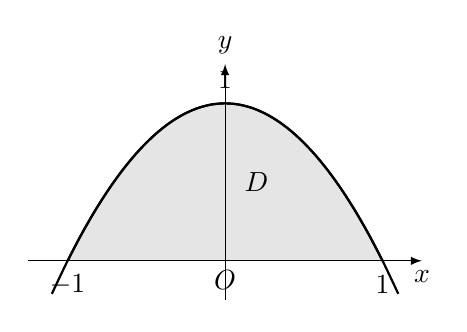
\begin{tikzpicture}[scale=2]
        \draw[black, thick, smooth, domain=-1:1,fill=gray!20] plot (\x, {-\x*\x+1});
        \draw[-latex](-1.25,0) -- (1.25,0) node[below]{$x$};
        \draw[-latex](0,-0.25) -- (0,1.25) node[above]{$y$};
        \filldraw[black] (0,0) node[below]{$O$};
        \draw[black](1,-0.15) node{$1$};
        \draw[black](-1,-0.15) node{$-1$};
        \draw[black](0,1.15) node{$1$};
        \draw[black, thick, smooth, domain=-1.1:1.1] plot (\x, {-\x*\x+1});
        \draw[black](0.2,0.5) node{$D$};
    \end{tikzpicture}
\end{minipage}

$f_X(x)=\dfrac{5}{4}\int_0^{1-x^2}x^2+y\,\textrm{d}y=\dfrac{5}{4}\left(x^2y+\dfrac{y^2}{2}\right)\bigg\vert_0^{1-x^2}=-\dfrac{5}{8}x^4+\dfrac{5}{8}$。

$f_Y(y)=2\dfrac{5}{4}\int_0^{\sqrt{1-y}}x^2+y\,\textrm{d}x=\dfrac{5}{2}\left(\dfrac{x^3}{3}+yx\right)\bigg\vert_0^{\sqrt{1-y}}=\dfrac{5}{6}(1-y)\sqrt{1-y}+\dfrac{5}{2}y\sqrt{1-y}$。

\subsubsection{二维均匀分布}

\subsubsection{二维正态分布}

概率密度为:

{\fontsize{8.2pt}{10pt}$f(x,y)=\dfrac{1}{2\pi\sigma_1\sigma_2\sqrt{1-\rho^2}}\exp\left\{-\dfrac{1}{2(1-\rho^2)}\left[\left(\dfrac{x-\mu_1}{\sigma_1}\right)^2-2\rho\left(\dfrac{x-\mu_1}{\sigma_1}\right)\left(\dfrac{y-\mu_2}{\sigma_2}\right)+\left(\dfrac{y-\mu_2}{\sigma_2}\right)^2\right]\right\}$}

其中$\mu_1,\mu_2\in R$,$\sigma_1,\sigma_2>0$,$-1<\rho<1$。

\paragraph{\boxed{\text{正态分布性质}}} \leavevmode \medskip

\textbf{例题:}$(X,Y)\sim N(\mu_1,\mu_2;\sigma_1^2,\sigma_2^2;0)$,分布函数为$F(x,y)$,已知$F(\mu_1,y)=\dfrac{1}{4}$,求$y$。

解:当$\rho=0$时,$F(X,Y)=\dfrac{1}{2\pi\sigma_1\sigma_2}e^{-\frac{1}{2}\left[\left(\frac{x-\mu_1}{\sigma_1}\right)^2+\left(\frac{y-\mu_2}{\sigma_2}\right)^2\right]}\\=F_X(x)F_Y(y)$,即$XY$相互独立。

$X\sim N(\mu_1,\sigma_1)$,$Y\sim N(\mu_2,\sigma_2)$,$F_X(\mu_1)=P\{X\leqslant\mu_1\}=\dfrac{1}{2}$。

$F(\mu_1,y)=F_X(\mu_1)F_Y(y)=\dfrac{1}{2}F_Y(y)=\dfrac{1}{4}$,则$F_Y(y)=\dfrac{1}{2}$,即根据性质$y=\mu_2$。

\paragraph{\boxed{\text{标准正态化}}} \leavevmode \medskip

$F(x)=P\{X\leqslant x\}=P\left\{\dfrac{X-\mu}{\sigma}\leqslant\dfrac{x-\mu}{\sigma}\right\}=\varPhi\left(\dfrac{x-\mu}{\sigma}\right)$。

即将$XY$的相关系数消去。

\textbf{例题:}设随机变量$(X,Y)$的分布函数为$\varPhi(2x+1)\cdot\varPhi(2y-1)$,其中$\varPhi(x)$为标准正态分布函数,求$(X,Y)$的分布函数。

解:由分布函数为$\varPhi(2x+1)\varPhi(2y-1)$是$X$的分布函数和$Y$的分布函数的乘积,所以可知$XY$相互独立。

所以根据标准化公式:$\varPhi(2x+1)\cdot\varPhi(2y-1)=\varPhi\left(\dfrac{x+\dfrac{1}{2}}{\dfrac{1}{2}}\right)\varPhi\left(\dfrac{y-\dfrac{1}{2}}{\dfrac{1}{2}}\right)$。

$\therefore(X,Y)\sim N\left(-\dfrac{1}{2},\dfrac{1}{2};\dfrac{1}{4},\dfrac{1}{4};0\right)$。

\paragraph{\boxed{\text{二维随机变量函数分布}}}

\subsubsection{离散型}

\subsubsection{连续型}

可以使用卷积公式法和分布函数法两种。

\paragraph{\boxed{\text{和的分布}}} \leavevmode \medskip

\textbf{例题:}随机变量$(X,Y)$的概率密度函数$f(x,y)=\left\{\begin{array}{ll}
    e^{-y}, & 0<x<y \\
    0, \text{其他}
\end{array}\right.$,求$P\{X+Y\leqslant1\}$。

解:根据$X+Y\leqslant1$和$0<x<y$划分区域:

\begin{multicols}{2}
    
    \begin{tikzpicture}[scale=2]
        \draw[-latex](-0.25,0) -- (1.25,0) node[below]{$x$};
        \draw[-latex](0,-0.25) -- (0,1.25) node[above]{$y$};
        \filldraw[black] (0,0) node[below]{$O$};
        \draw[black](1,-0.15) node{$1$};
        \draw[black](1,0) -- (0,1) node[left]{$1$};
        \draw[black](0,0) -- (1,1);
        \draw[black, densely dashed](0.5,0.5) -- (0.5,0) node[below]{$\dfrac{1}{2}$};
        \filldraw [fill=gray!20] (0.5,0.5) -- (0,1) -- (0,0) -- (0.5,0.5);
        \draw[black](0.2,0.5) node{$D$};
    \end{tikzpicture}

    其中积分区域$D$如图所示,所以$P\{X+Y\leqslant1\}=\iint\limits_De^{-y}\,\textrm{d}x\textrm{d}y=\int_0^{\frac{1}{2}}\textrm{d}x\int_x^{1-x}e^{-y}\,\textrm{d}y=\int_0^{\frac{1}{2}}(e^{-x}-e^{x-1})\textrm{d}x=1+e^{-1}-2e^{-\frac{1}{2}}$。

\end{multicols}

\paragraph{\boxed{\text{差的分布}}} \leavevmode \medskip

\textbf{例题:}设$X\sim N(\mu,\sigma_1^2)$,$Y\sim N(2\mu,\sigma_2^2)$,$XY$相互独立,已知$P\{X-Y\geqslant1\}=\dfrac{1}{2}$,求$\mu$。

解:若$X\sim N(\mu,\sigma_1^2)$,$Y\sim N(2\mu,\sigma_2^2)$,则$X-Y\sim(-\mu,\sigma_1^2-\sigma_2^2)$。则$X-Y$的均值为$-\mu$,即其图像的对称轴为$-\mu$。

又$P\{X-Y\geqslant1\}=\dfrac{1}{2}$,则$X-Y$在$1$这里均分,则对称轴为$1$,即$\mu=-1$。

\subsubsection{混合型}

使用全概率公式根据离散变量进行概率拆分。

\textbf{例题:}设随机变量$X_1$和$X_2$相互独立,已知$X_1\sim B\left(1,\dfrac{3}{4}\right)$,$X_2$的分布函数为$F(x)$,求$Y=X_1+X_2$的分布函数$F_Y(y)$。

解:已知$X_1\sim B\left(1,\dfrac{3}{4}\right)$,$X_2$的分布函数为$F(x)$,则$Y$为混合型。

则$P\{X_1=0\}=C_1^0\dfrac{3}{4}^0\dfrac{1}{4}^1=\dfrac{1}{4}$,$P\{X_1=1\}=C_1^1\dfrac{3}{4}^1\dfrac{1}{4}^0=\dfrac{3}{4}$。

$F_Y(y)=P\{X_1+X_2\leqslant y\}=P\{X_1+X_2\leqslant y|X_1=0\}P\{X_1=0\}+P\{X_1+X_2\leqslant y|X_1=1\}P\{X_1=1\}=P\{X_2\leqslant y|X_1=0\}P\{X_1=0\}+P\{1+X_2\leqslant y|X_1=1\}P\{X_1=1\}$,由相互独立性$=\dfrac{1}{4}\cdot P\{X_2\leqslant y\}+\dfrac{3}{4}\cdot P\{X_2\leqslant y-1\}$。

根据分布函数定义,则$F_Y(y)=\dfrac{1}{4}\cdot F(y)+\dfrac{3}{4}\cdot F(y-1)$。